\section{Human Integration}
In this section  there is a description of a mechanism that allow \textit{System0} to communicate with external reasoning and information retrieval services. These services to some extent imitate the creative process in human mind.\par
On some level of abstraction, association and attention are important concepts in human thinking process. Attention to an entity creates associations with it, and associations are the main mechanism to transfer attention. When we want to create a game plot we do not need to create a completely filled environment to simulate~-- all we need is to follow our associations. In imagination entities are created on demand and destroyed after there is no attention left to them. That is how we can drastically optimize the simulation process while using human mind based mechanisms.\par
Let us compare human mind creative process to the corresponding example based on \textit{Model0} in order to expand the later one to contain the former one's functionality.
The storyline-creator's activity can be decomposed into several smaller activities. To simplify the terminology these small activities will be referred as ``voices''. Let us consider the example voice set depicted in Figure~\ref{Voices}:
 \begin{figure}[h!]
    \begin{center}
      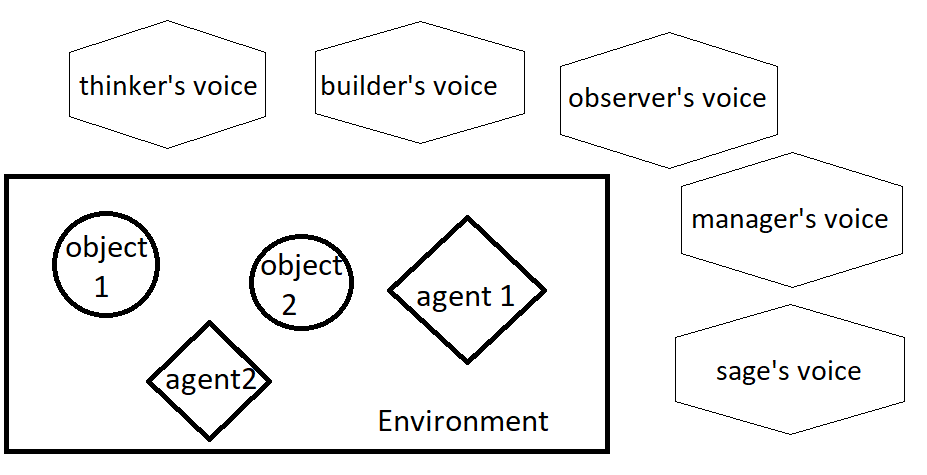
\includegraphics[width=300pt]{voices}
      \caption{The set of voices to be used to model human thinking process.}
      \label{Voices}
     \end{center}
    \end{figure}
\begin{itemize}
\item \textbf{The thinker's voice} is used to answer questions, for example, ``can a chicken fly?''.
\item \textbf{The builder's voice} is used to generate new entities and destroy the useless ones. Creates the chicken.
\item \textbf{The manager's voice} checks the simulations for exceptions and errors. Handles system's response on the flying chicken.
\item \textbf{The observer's voice} collects the most useful data for the final result. Creates the legend of the flying chicken.
\item \textbf{The sage's voice} retrieves requested information from a knowledge base. States that usually chickens can not fly, but they are yellow, small, and produce the sound, contained in \texttt{``chicken\_sound.mp3''}.
\end{itemize}
Each of this voices can be supplemented to \textit{Model0} as interface that can either be automated or used to transfer information between human and simulation. In terms of simulation framework this voices may correspond to the following classes:
\begin{itemize}
\item \textbf{GameThinkerVoice} is called whether there is no method defined to handle an event.
\item \textbf{GameBuilderVoice} is used to fill the environment with appropriate \texttt{GameObjects}, \texttt{GameAgents}, \texttt{GameEnvironmentObjects} and \break \texttt{GameEnvironmentAgents}. Also it can dynamically add properties. To separate these 2 activities it can be divided in 2 voices: \texttt{GameCreatorVoice} and \texttt{GameRefinerVoice}.
\item \textbf{GameManagerVoice} coordinates the actions of another voices. Handles errors in case other voices are malfunctioning. Also it can be responsible for pausing, stopping, and restarting the simulation.
\item \textbf{GameObserverVoice} retrieves and processes useful simulation data while having full access to every bit of information in the simulation.
\item \textbf{GameSageVoice} is used whether there is a need to define any properties of an entity.
\end{itemize}
Messages to the voices can be either sent by \texttt{GameAgents}, \texttt{GameEnvironments} or by another voices. Messages from the voices bypass the standard \texttt{GameEnvironment} $correct$ procedure.
\begin{definition}
\textbf{Model0V} is an extension of \textit{Model0} that is created by including voice classes described earlier. In other words,
\textit{Model0V} = \textit{Model0}  + Voices.
\end{definition}

